\chapter{CARACTERÍSTICAS TÉCNICAS DA PLATAFORMA \textit{RASPBERRY PI}}

\textit{Raspberry Pi} é um computador do tamanho de um cartão de  rédito desenvolvido no Reino Unido pela Fundação \textit{Raspberry Pi} com a intenção de estimular o ensino de informática básica nas escolas. Ele se conecta à sua TV e a um teclado, e pode ser usado para muitas das coisas que o seu PC \textit{desktop} faz, como processar textos, planihas e jogos, além de reproduzir vídeo de alta definição. Todo o \textit{hardware} é integrado em uma única placa, e o projeto é baseado em um \textit{system on a chip} (SoC) Broadcom BCM2835, que inclui um processador ARM1176JZF-S de 700 MHz, GPUVideoCore IV, e 512 MB de memória RAM em sua última revisão. O projeto não inclui uma memória não-volátil - como um disco rígido - mas possui uma entrada de cartão SD para armazenamento de dados. A placa é adaptada para rodar sistemas operacionais baseados em Linux \cite{WIKIPEDIA2}.

\subsection{História}

A ideia de criar um computador pequeno e barato para crianças surgiu em 2006, quando Eben Buton e seus colegas da Universidade de Cambridge perceberam que os estudantes de hoje que querem estudar ciência da computação não têm as habilidades que eles tinham na década de 1990. Eles atribuem isso, entre outros fatores, à ascensão do computador pessoal (PC) e dos \textit{consoles} de jogos que substituíram os microcomputadores. Desde que o computador tornou-se importante para todos os membros da família, o ato de deixar os membros mais jovens brincarem ou fazerem experimentos foi sendo cada vez mais desestimulado.

Mas recentemente os processadores usados em telefones celulares e tablets tornaram-se mais baratos e mais poderosos, abrindo caminho para o lançamento do \textit{Raspeberry Pi} no mundo das placas de computadores ultrabaratas e úteis.

\subsection{Viabilidade no mercado brasileiro}

Para se obter um \textit{Raspberry Pi} no Brasil é preciso importá-lo. No site da farnellwark, empresa que realiza serviços de importação e revenda, o valor da placa \textit{Raspberry Pi} - Modelo B é R\$ 176,02. O preço apresentado anteriormente é um somatório do custo real da placa com despesas referentes à importação, sendo que o frete para a entrega do equipamento em sua residência ainda não está incluso. Para se ter uma noção do aumento no valor da compra gerado pela despesas com importação, foi pesquisado o preço em um site que vendesse a mesma placa sem tais custos. No site da adafruit, o preço encontrado foi de \$ 39,95, o equivalente a R\$ 88,61, de acordo com a cotação do dólar às 12h do dia 21 de setembro de 2013, evidenciando assim uma diferença de R\$ 87,49.

\begin{table}[!htpb]
 \centering
    \begin{tabular}{|l|p{3cm}|c|} 
    \hline
        \textbf{Valor} & \textbf{Impostos} & \textbf{Valor Total} \\
    \hline
        R\$ 90,93 & R\$ 87,49 & R\$ 176,02 \\
    \hline
    \end{tabular}
    \caption{Apresentação do valor do \textit{Raspberry Pi} agregado com gastos de importação para o Brasil. O valor total não inclui o frete.}
    \label{t_fixa}
\end{table}

O frete e o tempo de entrega do equipamento em residência varia de acordo com a localidade da mesma. Para uma entrega em Campos dos Goytacazes, o valor do frete cobrado foi de R\$ 32,20 e o tempo de 3 dias úteis.

Em relação a empresas que oferecem suporte à placa no Brasil não foi encontrada nenhuma informação.

\subsection{Comparativo de custos de \textit{hardware} semelhante}

Para apresentar a diferença de custo entre o \textit{Raspberry Pi} e um \textit{hardware} semelhante, mais precisamente um computador \textit{desktop}, foram escolhidas duas empresas para serem alvos da pesquisa de preço. A primeira será a Farnell Newark, empresa já apresentada na seção anterior e que fornecerá o valor do \textit{Raspberry Pi}, e a segunda será a Americamas.com, empresa que informará o preço do PC \textit{desktop} mais barato existente na loja. Em ambas as empresas tal pesquisa de preço foi realizada às 14:18 horas do dia 28 de setembro de 2013.

O valor apresentado pela Farnell Newark para o \textit{Raspberry Pi} foi de R\$ 176,02 mais despesas com frete, enquanto que a loja Americanas.com vende o pc \textit{desktop} mais barato pelo preço de R\$ 719,00.

Ao se analisar os valores apresentados no parágrafo anterior, é preciso entender que a comparação entre os equipamentos não acontece em torno da capacidade de seus componentes, tais como poder de processamento, quantidade de memória RAM, capacidade de disco rígido, e etc, pois se assim fosse o pc \textit{desktop} desbancaria a nova tecnologia que está sendo apresentada. O objetivo do comparativo está em mostrar o bom custo x benefício que o  \textit{Raspberry Pi} pode apresentar.

\subsection{Sistemas computacionais que utilizam o \textit{Raspberry Pi}}

Apesar de os idealizadores do \textit{Raspberry Pi} o terem criado visando uma prática maior da programação entre jovens e crianças, o equipamento tem sido utilizado por pessoas do mundo inteiro a fim de alcançarem outros objetivos. Sendo assim, foram pesquisados projetos que apresentassem exemplos do uso do equipamento em sistemas computacionais, e o resultado a seguir.

Em um artigo escrito por \citeonline{PEDRO}, o \textit{Raspberry Pi} é utilizado como um servidor de \textit{Virtual Private Network} (VPN) ou Rede Privada Virtual. Após demonstrar passo a passo a instalação de alguns pacotes e realizar algumas configurações necessárias, o autor do artigo explica que ao se conectar a uma rede pública e necessitar da garantia que a sua conexão é segura, pode-se fazer uso do \textit{Raspberry Pi} para que as conexões sejam cifradas e que passe por ele.

Segundo \citeonline{ZACH}, é possível fazer do \textit{Raspberry Pi} um servidor web barato para realizar testes ou armazenar arquivos.

Nota-se então que já se encontram exemplos de sistemas computacionais baseados no \textit{Raspberry Pi}, o que multiplica as possíveis utilidades dessa nova tecnologia.

\subsection{Descrição técnica}

\begin{figure}[ht]
    \centering
    \scalebox{0.41}{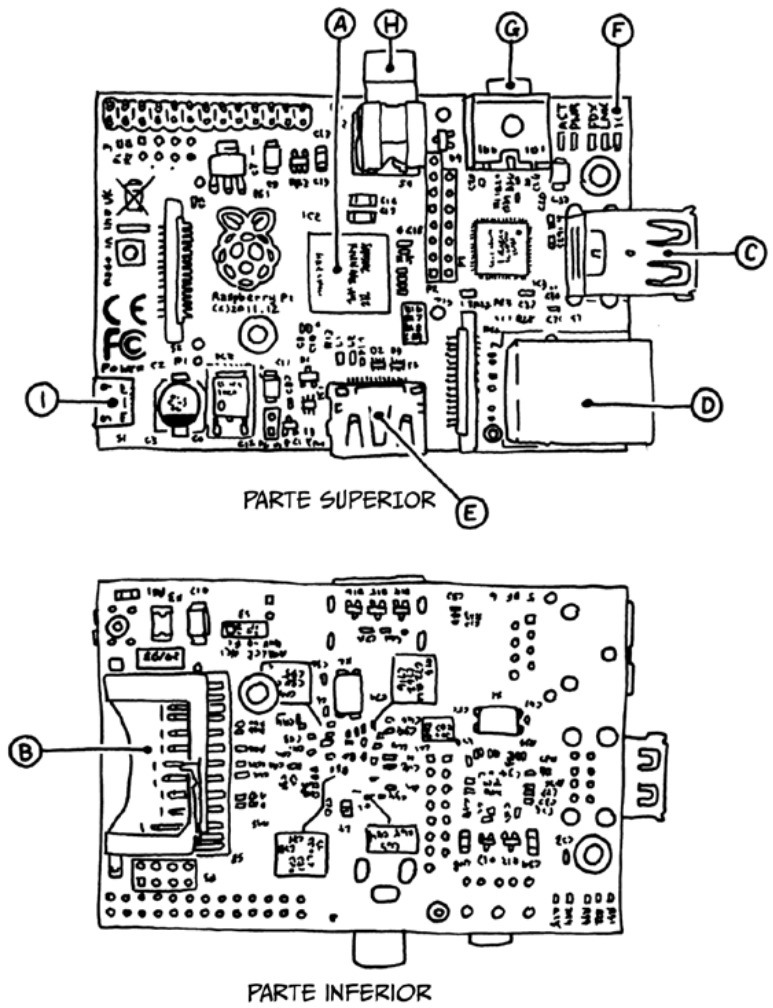
\includegraphics{figuras/superior_inferior}}
    \caption{Ilustração da placa \textit{Raspberry Pi}}
\end{figure}

A Figura 4.1 representa a placa do computador \textit{Raspberry Pi} contendo indicações em diversos componentes, os quais serão melhor especificados a seguir.

\textbf{A. Processador.} No coração do \textit{Raspberry Pi} está o mesmo processador que você encontraria no iPhone 3G e no Kindle 2, assim você pode pensar nas capacidades do \textit{Raspberry Pi} como comparáveis a esses poderosos pequenos aparelhos. Este processador trabalha na frequência de 700 MHz - 32 bits, e foi construído sobre a arquitetura ARM11. Chips ARM apresentam-se em uma variedade de arquiteturas com diferentes núcleos configurados para fornecer diferentes capacidades com preços diferentes. O modelo B tem 512 MB de memória RAM e o modelo A tem 256 MB. (O primeiro lote do modelo B tinha apenas 256 MB de RAM.)
    
\textbf{B. Slot para cartão de memória SD (Secure Digital).} Você perceberá que não há disco rígido no Pi; tudo é armazenado em um cartão de memória SD. Uma razão pela qual você irá desejar, mais cedo ou mais tarde, algum tipo de gabinete (case) de proteção, é que as soldas no soquete SD poderão quebrar se o cartão for acidentalmente dobrado.

\textbf{C. Porta USB.} No modelo B há duas portas USB 2.0, mas apenas uma no modelo A. Algumas das primeiras placas do \textit{Raspberry Pi} foram limitadas quanto à quantidade de corrente que elas poderiam fornecer. Alguns dispositivos USB podem chegar a 500mA. A placa original do Pi suportava 100mA ou quase, mas as revisões mais recentes alcançam até a especificação completa das portas USB 2.0. Provavelmente não é uma boa ideia recarregar seu celular com o \textit{Raspberry Pi}. Você poderá usar um hub com alimentação externa se tiver um periférico que necessite de mais energia.

\textbf{D. Porta Ethernet.} O modelo B tem uma porta Ethernet padrão RJ45. O modelo A não tem, mas pode ser conectado a uma rede com fios por meio de um adaptador de rede Ethernet USB (a porta no modelo B é na verdade um adaptador Ethernet USB embutido). A conectividade Wi-Fi por meio de um adaptador USB externo é outra opção.

\textbf{E. Conector HDMI.} A porta HDMI oferece saída de áudio e vídeo digital. Catorze resoluções de vídeo diferentes são suportadas, e o sinal HDMI, por meio de adaptadores externos, pode ser convertido para DVI (usado por muitos monitores), vídeo composto (sinal de vídeo analógico normalmente transmitido por um conector RCA amarelo), ou SCART (uma norma europeia para conexão de equipamentos audiovisuais).

\textbf{F. LEDs de status.} O Pi tem cinco LEDs indicadores de status que podem ser visualizados na Tabela 4.1 abaixo.

\begin{table}[!htpb]
 \centering
    \begin{tabular}{|l|p{2cm}|l|} 
    \hline
        \textbf{Led} & \textbf{Cor} & \textbf{Descrição} \\
    \hline
        ACT & Verde & Acende quando o cartão SD é acessado \\
    \hline
        PWR & Vermelho & Conectado à alimentação de 3.3V \\
    \hline
        FDX & Verde & On (ligado) se o adptador de rede é full-duplex \\
    \hline
        LNK & Verde & Luz indicando atividade de rede \\
    \hline
        100 & Amarelo & On (ligado) se a conexão de rede for 100Mpbs \\
    \hline
    \end{tabular}
    \caption{LEDs com cindo indicações de status}
    \label{t_fixa}
\end{table}

\textbf{G. Saída de áudio analógico.} É um conector de áudio analógico padrão de 3,5 mm que é destinado a conduzir cargas de alta impedância (como alto-falantes amplificados). Fones de ouvido ou alto-falantes sem alimentação não terão som de qualidade. Parte desse problema tem a ver com o software controlador de áudio, o qual ainda está em desenvolvimento.

\textbf{H. Saída de vídeo composto.} É um conector-padrão tipo RCA que fornece sinais de vídeo composto NTSC ou PAL. Esses formatos de vídeo têm resolução extremamente baixa se comparada com HDMI. Se você tiver um monitor ou um televisor com entrada HDMI, use-o em vez de um televisor com entrada de vídeo composto.

\textbf{I. Entrada de energia.} Uma das primeiras coisas que você perceberá é que não há nenhum interruptor de alimentação no \textit{Raspberry Pi}. Esse conector micro USB é usado para fornecer energia (essa não é uma porta USB adicional, é apenas para alimentação). A porta micro USB foi escolhida porque o conector é barato e fontes de alimentação USB são fáceis de encontrar.

\newpage

\subsection{Periféricos adequados}

Após adquirir-se um pouco de conhecimento sobre os componentes da placa, faz-se necessário saber também sobre os periféricos adequados para utilizar com ela. A imagem abaixo mostra alguns dos quais iremos precisar para utilizar o \textit{Raspberry}. É preciso tomar cuidado, pois existem peças que podem não funcionar corretamente quando instaladas na sua placa.

\begin{figure}[ht]
    \centering
    \scalebox{0.27}{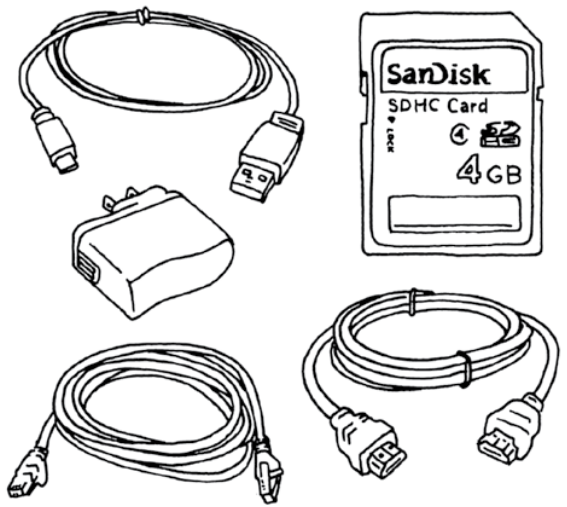
\includegraphics{figuras/perifericos_adequados}}
    \caption{Periféricos básicos: uma fonte de alimentação micro USB, cabos e cartão SD.}
\end{figure}

\textbf{Fonte de alimentação.} Este é o periférico mais importante para ser obtido. Você deve usar um adaptador micro USB que pode fornecer 5V e pelo menos 700mA de corrente (500mA para o modelo A). Um carregador de telefone celular não vai funcionar, mesmo se ele tiver o conector correto. Um carregador de telefone celular típico fornece apenas 400mA de corrente ou menos, mas verifique a classificação indicada na parte de trás. Um \textit{Raspberry Pi} com fonte de alimentação inferior pode parecer funcionar, mas ficará estranho e poderá falhar (travar) de forma imprevisível. Um problema comum causado por insuficiência de corrente descrito pelos usuários do \textit{Raspberry Pi} é que o teclado não funciona corretamente.

\textbf{Cartão SD.} Você vai precisar de pelo menos 4GB, e deve ser um cartão de Classe 4. Estes cartões são capazes de transferir pelo menos 4MB/seg. Algumas das placas anteriores do \textit{Raspberry Pi} apresentaram problemas com cartões de Classe 6 ou superiores, os quais são capazes de velocidades mais rápidas, mas com menos estabilidade. Um cartão micro SD em um adaptador é perfeitamente utilizável também.

\textbf{Cabo HDMI.} Se você está se conectando a um monitor, precisará deste cabo ou um adaptador apropriado para um monitor DVI. Você também pode executar o Pi sem monitor, como descrito posteriormente neste capítulo. Cabos HDMI podem variar muito de preço. Se está instalando um cabo de 90 a 180 cm para o monitor, não há necessidade de gastar mais de US\$ 3 em um cabo HDMI. Se estiver instalando comprimentos maiores, você definitivamente deve pesquisar cabos de maior qualidade e evitar os genéricos mais baratos.

\textbf{Cabo Ethernet.} Visto que atualmente praticamente tudo é sem fio (wireless), você pode encontrar um pouco de dificuldade com a porta com fio (cabeada).

\subsection{Outras características}

O \textit{Raspberry Pi} ainda apresenta outras características, sendo capaz de imprimir em impressora local e em rede, servir arquivos em rede, executar as linguagens de programação java, ruby e python, além de editar textos, planilhas e apresentações.